%%%%%%%%%%%%%%%%%%%%%%%%%%%%%%%%%%%%%%%%%%%%%%%%%%%%%%%%%%%%
%%%%%%%%%%%%%%%%%%%%%%%%%%%%%%%%%%%%%%%%%%%%%%%%%%%%%%%%%%%%
\chapter{Protein Sequencing by MS/MS}
\nopagebreak
\label{chap:msms}
%%%%%%%%%%%%%%%%%%%%%%%%%%%%%%%%%%%%%%%%%%%%%%%%%%%%%%%%%%%%
%%%%%%%%%%%%%%%%%%%%%%%%%%%%%%%%%%%%%%%%%%%%%%%%%%%%%%%%%%%%

Tandem mass spectrometry (MS/MS) is used in order to produce structural information about
a compound by fragmenting-specific sample ions inside the mass spectrometer and
identifying the resulting fragment ions.
This information can then be pieced together to generate structural information
regarding the intact molecule. 
Tandem mass spectrometry also enables specific compounds to be detected in
complex mixtures on account of their specific and characteristic fragmentation
patterns.
In proteomics, MS/MS represents a useful instrument to identify 
the primary structure (i.e., the amino-acid sequence) of the proteins
contained in  the target sample.

A tandem mass spectrometer is a mass spectrometer that has more than one
analyser, in practice usually two.
The first mass analyser (MS$_1$) is used to select user-specified sample ions (\emph{precursor
ions}) arising from a particular component; usually ions associated to the whole molecule 
(i.e. (M+H)$^+$ or (M-H)$^-$ ions).
The selected ions pass into the collision cell, where they are bombarded by the
inert gas molecules which cause fragment ions to be formed (\emph{product ions}).
The latter are analysed, i.e. separated according to their mass to charge
ratios, by the second analyser (MS$_2$).
The resulting product ions arise directly from the precursor ions specified in the
experiment, and thus produce a fingerprint pattern specific to the compound
under investigation.
This type of experiment is particularly useful for providing structural
information concerning small organic molecules and for generating peptide
sequence information.
In the latter case, which is the one of interest here, 
the precursors ions are those obtained by enzymatic digestion of an
unidentified protein, which typically yields small polypeptides of length ranging
between a few and a few tens of amino-acids. Their separation according to their
mass, and successive fragmentation into all possible pairs of N- and C-term
pieces, provides, in principle, the full information to enable the readout of
the sequence from the resulting fragment spectrum, as explained in the following sections.

%%%%%%%%%%%%%%%%%%%%%%%%%%%%%%%%%%%%%%%%%%%%%%%%%%%%%%%%%%%%
\section{The Sequencing Workflow}
%%%%%%%%%%%%%%%%%%%%%%%%%%%%%%%%%%%%%%%%%%%%%%%%%%%%%%%%%%%%
\subsection{Separation and Digestion}

In a typical proteomics experiment a sample with a complex mixture of protein
(for instance, resulting from a cell lysate, and providing a snapshot of
the proteome of the cell at the moment of its disruption) has to be analysed. 
The first step for identification and quantitation of the different proteins
contained in the mixture is to separate them from each other, to allow
individual processing.

The separation of the sample mixture is usually performed by 2-D gel
electrophoresis, producing numerous samples in which there is usually only one
dominant protein, even if other molecules
and protein can be present at very low concentration. 
In other words, each spot can be considered as an ensemble of identical protein,
if we neglect the above mentioned impurities.
Once separated, the proteins undergo a enzymatic digestion usually accomplished %carried on
by %the protein 
Trypsin.

Trypsin is an enzyme  with a catalytic pocket that specifically cleaves the
polypeptide on the carboxyl side of the amino-acids Lysine (K) or Arginine (R).
The cleavage is inhibited if the Lysine or the Arginine are followed by a
Proline (P).
Although other enzymes can be used to cut the protein into smaller peptides, the
above rules make trypsin the most useful and common enzyme for digesting
proteins: indeed, due to the natural frequency of the K and R amino acids in
protein sequences, the above cleaving rules produce  a specific length
distribution for the tryptic cleavage, with only 10\% of fragment longer than 20 residues, while keeping a
reasonable low concentration of short residues.

%%%%%%%%%%%%%%%%%%%%%%%%%%%%%%%%%%%%%%%%%%%%%%%%%%%%%%%%%%%%%%%%%%5
\subsection{Ionization}

Mass Spectrometry relies on the availability of simple ionizations techniques
and accurate measurement instrumentation.
The most popular ionisation methods available (see
\cite{ashcroft1997ionization-methods} and references cited therein)
are Electrospray Ionization (ESI) and Matrix Assisted Laser Desorption
Ionization (MALDI). Other methods include Atmospheric Pressure Chemical
Ionisation, Chemical Ionisation, Electron Impact, Fast Atom Bombardment, Field
Desorption and Field Ionisation, Thermospray Ionisation.

Indeed, the development of Electrospray
Ionization \cite{fenn1989,dewald1999} and Matrix-assisted Laser Desorption Ionization
\cite{hillenkamp1991} prompted for important developments in mass spectroscopy
instrumentation that would revolutionize protein chemistry and protein analysis
during the decade of the nineties.

The above methods generate ions from large, non-volatile analytes such as proteins and
peptides without significant analyte fragmentation.
For this ionization characteristic they are also referred to as "soft" ionization methods.
(in fact they are so soft that under specific conditions
even non-covalent interactions may be maintained
during the ionization process.)

Due to the pre-eminence of this two methods, we discuss them in more detail in the following.


\paragraph{Electrospray Ionization.}
ESI popularity raised in part due to the ease with which it could
be interfaced with popular chromatographic and
electrophoretic liquid-phase separation techniques necessary to produce almost
pure protein samples.
This ionization method, then, displaced previous popular methods 
such as fast atom bombardment for protein and
peptide samples dissolved in a liquid phase.

During standard ESI \cite{fenn1984electrospray}, 
the sample is dissolved in a polar, volatile solvent and pumped through a narrow
%, stainless steel,
capillary. 
A high voltage 
%of 3 or 4 kV 
is applied to the tip of the capillary where, as a consequence of
this strong electric field, the sample emerge and disperse in form of the
aerosol of highly charged droplets.
A gas flow, usually nitrogen, helps to direct the spray emerging from the capillary tip towards the
mass spectrometer. 
The nitrogen warm flow, also known as drying gas, helps the evaporation of the
solvent causing the droplets to diminish in size. 
The charged ions trapped in the decreasing-in-size droplets, manage to escape
and pass through a sampling cone into an intermediate vacuum region, and from
there, through a small hole, into the first analyser of the mass spectrometer, which
is kept in  high vacuum conditions.
%The lens voltage is optimized individually for each sample.

The ionization of proteins and peptides is usually positive while
for saccharides and oligonucleotides ionization is negative.
In all
cases, the $m/z$ scale must be calibrated by analysing a standard sample,
similar to the target sample being analysed, and then a mass correction must by
applied.

The sample ions usually are produced in a singly charged state that in positive
ionization, the one we are interested in, means protonated molecular ions
$(M+H)^+$ (while negative ionization give rise to deprotonated molecular ions).
High values of peptide mass, exceeding 1200 Da., can give rise to multiply
charged ions $(M+nH)^{n+}$\cite{Takats2004}.

%Using electrospray or nanospray ionisation, a mass accuracy of within 0.01\% of the molecular mass
%should be achievable, which in this case represents $\pm 1.4$ Da. (???)


\paragraph{MALDI.}
MALDI is the other popular ionization method, although for different reasons.
This ionization method is commonly used coupled to the time-of-flight (TOF)
analyser, that we will talk about later on, that is robust, simple, and
sensitive, with a large mass range. 
MALDI ionization method produce ions which generally are singly charged,
simplifying, thus, the interpretation task.
% The method is relatively resistant to 
% interference with matrices commonly used in protein chemistry.


MALDI \cite{hillenkamp1991maldi} deals well with proteins and other
thermolabile, non-volatile organic compounds, especially
those of high molecular mass.
% and is used successfully in biochemical areas for
%the analysis of
%peptides, glycoproteins, oligosaccharides, and oligonucleotides. 
%It is relatively straightforward to use and reasonably tolerant to buffers and other additives.
The mass accuracy depends on the type and
performance of the analyser of the mass spectrometer, but most modern instruments should be capable of
measuring masses to within 0.01\% of the molecular mass of the sample.
In MALDI, the sample is co-crystallised with an highly absorbing organic matrix
compound, this usually contain an aromatic ring that can absorb the wavelength
of a laser. 
The laser bombardment is transformed into energy by the matrix compound and then
particles of the mixture of matrix compound and analyte ions are released from the surface.


The calibration of the spectrometer scale is performed, usually, with a known sample that can either be analysed
independently (external calibration) or pre-mixed with the sample and matrix (internal calibration).
MALDI is also a "soft" ionisation method and the predominant products are
protonated  molecular ions (M+H$^+$) regardless of the molecular mass.
Traces of doubly charged ions at approximately half the $m/z$ value can be found.


%%%%%%%%%%%%%%%%%%%%%%%%%%%%%%%%%%%%%%%%%%%%%%%%%%%%%%%%%%%%%%%%%%%%%%%
\subsection{Analysers}

After the ionization of the sample molecular ions, these have to be separated
and their mass-to-charge ration measured.
A variety of analysers are used to this scope, the most commons are are
Quadrupole mass analyser, Magnetic sector and Time Of Flight (TOF).

\paragraph{Quadrupole Mass Analyser.}
This analyser consist of four parallel rods. Opposing rods are paired together
and connected electrically: a variable potential is applied between
the two pair of rods with radio frequency oscillations, while a time-independent
potential is superimposed.
The injected ions are affected by the oscillating electrical potential and the
beam is alternatively focused toward the centre and dispersed toward the rods in
both directions perpendicular to the rods axis.
The superimposed constant potential, say positively biasing the rod pair 1, and
negatively biasing the rod pair 2, acts as a mass filter in the two dimension:
if positively biased, the heavier ions (suppose positive ions) are affected by
the average potential and focused toward the centre of the quadrupole, lighter
ions, affected by the rapidly varying potential, experience large accelerations
toward the rods and are eliminated from the beam, creating a high pass mass
filter;
on the other axis, with negative biased potential, the heavier ions are
attracted by the average negative rods potential, while in lighter ions this
behaviour is contrasted by the oscillating potential, this a low pass mass
filter.
The combination of the two filters result in a band pass mass filter that select
ions based on their mass-to-charge ratio. The band width is related to the
instrument mass resolution\cite{Miller1986}.


\paragraph{Magnetic Sector}
The behaviour of ions in a homogeneous, linear, static magnetic field
as in a sector instrument is simple. The physics are
described by the Lorentz force law in the case of zero electric field:
\begin{equation}
    \mathbf{F} = q \mathbf{v} \times \mathbf{B}
\end{equation}
where $\mathbf{B}$ is the magnetic field induction, $q$ is
the charge of the particle, $\mathbf{v}$ is its current velocity.
In this case the molecular ions are accelerated by a electrical potential $V$
and
then injected into the magnetic field, the forces experienced by the particles
are perpendicular to the trajectory resulting in a arc of square radius
$r^2=\frac{2V}{B^2}\frac mz$.
Given then the accelerating potential $V$ and the magnetic field inside the
magnetic sector $B$, then the radius of the trajectory only depends on the
mass-to-charge ratio of the travelling particle.


\paragraph{Time Of Flight}
Time-of-flight mass spectrometry (TOF) is a method of mass spectrometry in
which ions $\frac mz$ ratio is determined via a time measurement. 
Ions are accelerated by an electric field $\mathbf{E}$ of known strength:
\begin{equation}
    \mathbf{F} = q \mathbf{E}
\end{equation}
this results in an ion acceleration and a velocity that depends only on 
the mass-to-charge ratio. 
The time that it takes to reach the detector at a known
distance is measured and will depend on the $m/z$ ratio of the
particle. 





%%%%%%%%%%%%%%%%%%%%%%%%%%%%%%%%%%%%%%%%%%%%%%%%%%%%%%%%%%%%%%%%%%5
\subsection{Collision-Induced Dissociation and Product Detection}
\label{subsec:cid-spectrum}

\begin{figure}
\centering
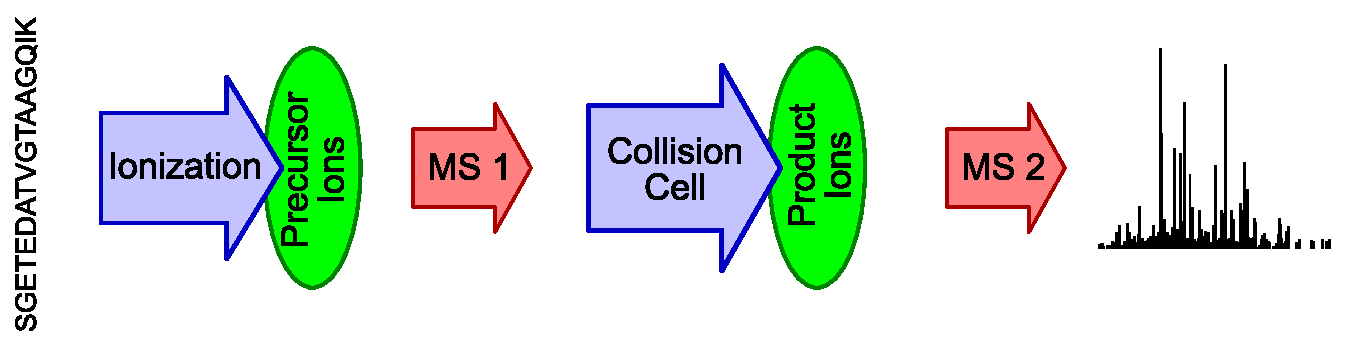
\includegraphics[width=0.9\textwidth]{./img/msms/msms-scheme.eps}
\caption{\label{fig:msms-scheme}
MS/MS scheme. The protein, once purified and digested by Trypsin, undergoes
ionization through MALDI or ESI, the resulting precursor ions are separated
in the first analyser MS$_1$. A selected precursor ions is fragmented in the CID
(see text) and the resulting product ions are separated by the second analyser
MS$_2$ to be recollected in the experimental spectrum on the basis of their
mass-to-charge ratio.}
\end{figure}


So far, the peptides, produced from the enzymatic digestion of an ensemble of
identical proteins, have been separated according to their mass/charge ratio in
the first MS analyser. The determination of their masses can be sufficient for
the identification of the protein by peptide fingerprinting, as described in the
previous chapter, provided that a protein database containing its sequence is
available, and the identification is not hindered by post-translational
modifications that change the mass of the ``bare'' peptide. However, to proceed
further towards a true sequencing of each peptide, a mechanism is needed to
resolve the individual amino-acid residues that compose the peptide. To this
end, Collision Induced Dissociation is combined to a second MS analyser,
according to the following protocol (see Fig.~\ref{fig:msms-scheme} for a scheme
of the process)..

The molecular ions that travel from the first analyser are
accelerated by some electrical potential to high kinetic energy in the vacuum of
the mass spectrometer and then allowed to collide with neutral gas molecules
(often helium, nitrogen or argon). In the collision some of the kinetic energy
is converted into internal energy which results in bond breakage and the
fragmentation of the molecular ion into smaller fragments. 
whose number depends on the energy involved in the collision. Typically,
low-energy CID (the one that we will deal with in more detail) split the
``parent peptide'' in two fragments, a N-terminal and a C-terminal one, while
high-energy CID can yield internal fragments, braking the parent peptide in more
than one point.

While CID is currently the most popular method for standard tandem
mass spectrometry, there are other also other fragmentation methods for special
purposes, for example electron-transfer dissociation (ETD), electron-capture
dissociation (ECD), and infra-red multi-photon dissociation (IRMPD). Alternative
fragmentation methods are particularly useful for identification of
phosphorylation sites and other post-translational modifications
(PTMs).
% (see page~\pageref{ptms}).

Peptides fragment in a reasonably well-documented manner
\cite{roepstorff1984nomenclature,johnson1989interpretation} even if the
underlying physics is not completely understood, and it is not feasible, at the
moment, to predict the outcoming distribution of charged and neutral fragments,
since they depend not only on the composition but also on the conformational
state of the peptide during the
collision\cite{dancik1999,gygi2004nature,Wan2006,Zhang2004}. 
Fragmentation generally occurs between two consecutive residues, breaking a
peptide bond on the main chain of the peptide, this can happen in three different ways generating three
corresponding pairs of fragments (see Fig.~\ref{fig:frag}).
The first fragmentation site is localised on the bond between the $C_\alpha$ carbon
and the subsequent $C=O$ of the same residue while the proton carrying the
positive charge could be alternatively associated to the N-terminal fragment,
giving rise to an $a$ type ion, or to the C-terminal fragment, giving rise to a
$x$ type ion.
The second fragmentation site is between the C-terminal of the carboxyl group of a
residue and the amino group of the following residue, giving rise to the $b$
and $y$ type ions for the N and C-terminal parts respectively.
Last fragmentation site can be found between the amino group and the $C_\alpha$
carbon of the same residue, giving rise to $c$ and $z$ ions.
\cite{roepstorff1984nomenclature,Johnson1987}
Only the fragments carrying the charge inherited from the precursor ion produce
an event on the resulting spectrum.
While the resulting distribution of ions is not predictable, ions labelled $b$
and $y$ are the most observed.

\begin{figure}
\centering
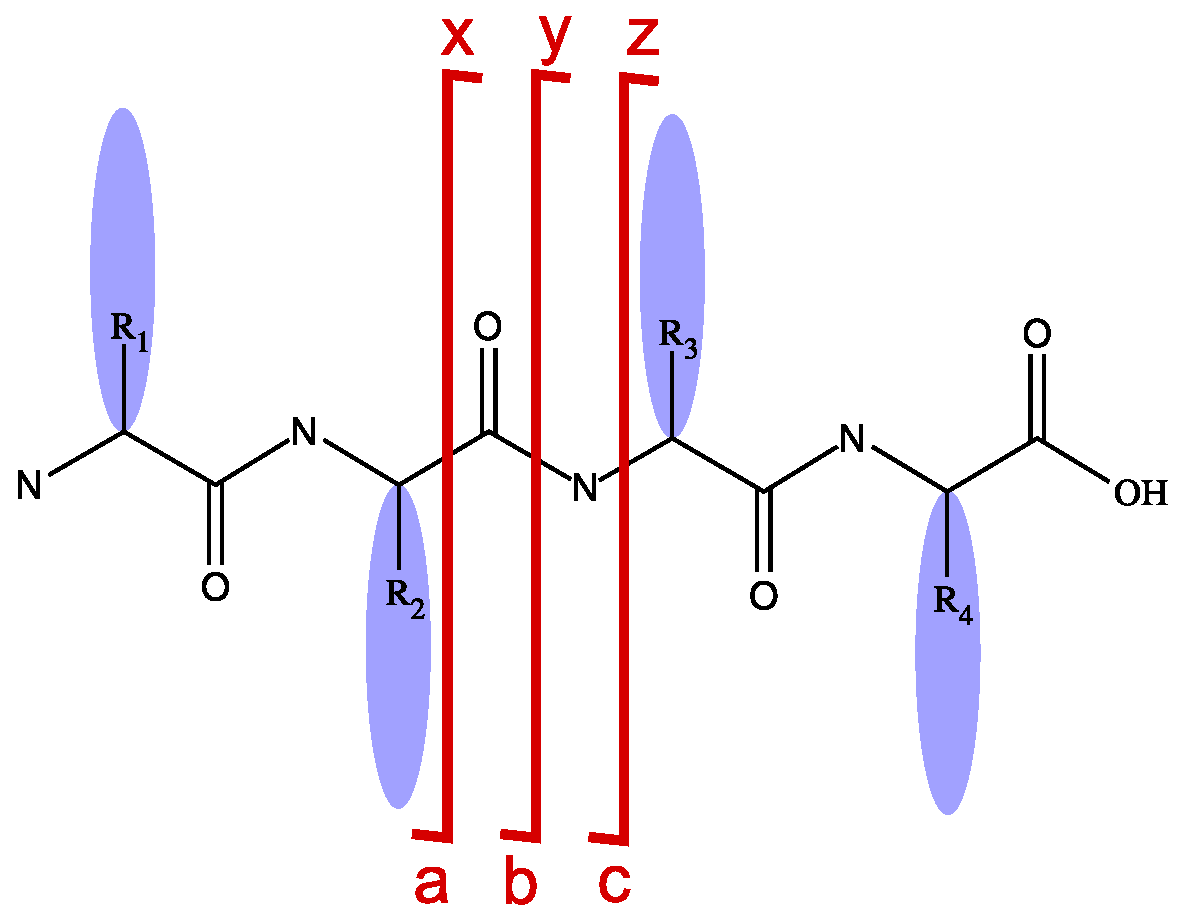
\includegraphics[width=7cm]{./img/msms/amino-cleavage.eps}
\caption{\label{fig:frag}Peptide fragmentation scheme. Ions families
produced by the CID fragmentation of the precursor ions, distinguished by
fragmentation pattern.
Fragments $a,b$ and $c$ are the N-term part of the fragmentation in the NH-CH,
CH-CO, and CO-NH bonds respectively, while $x,y$ and $z$ correspond to the
C-terminal part of the same fragmentations. }
\end{figure}


To make things more difficult, during collisions the fragment ions can undergo
neutral losses (loosing, for instance, water or ammonia groups) or accept more charges
depending on the precursor charge state depending on the residues composing the
resulting ion.
If the precursor ion is carrying more than one charge, the outcoming singly
charged ions can accept a further proton increasing its charge state if the ion
contain at least a Lysine (K), an Arginine (R) or a Histidine (H), this results
in a observed peak at half the joint mass of the product ion and the proton.
Some residues, during the collision dissociation can loose a neutral group,
the most common neutral groups are water (lost by Serine (S) and Threonine (T))
that results in a second peak shifted by -18.01 Da. from the original peak,
ammonia (Glutamine (G), K, R) with a peak shift of -17.03 Da., and urea (R) with
a peak shift of -97.98; while H and R can accept a water group resulting in a
new peak shifted by +18.01 Da..

Another difficulty source for a straight spectrum interpretation is the presence
in the observed ions of elements with high isotopes content, such as carbon and
nitrogen, the highest peaks are then often accompanied by isotopes peaks shifted
by 1 Da. that become important for bigger ion masses. It is feasible that more
than one isotope peak is found if heavier ions are presents.

%\subsection{interpretation}
The resulting charged fragments are detected by the second MS analyser, and add
up to the parent peptide spectrum.
If  fragmentations at every position along the sequence were equally likely, and
if no noise from impurities or contaminants were present, the resulting spectrum
would consist of a series of N-series and C-series peaks, of equal intensity, as
in Fig.~\ref{fig:spectrum-teo}.
The determination of the sequence would be possible by simply reading out the
masses of the component residues from the difference in the position of the
peaks along the $m/z axis$. However, things are more complicated than that, and
a typical spectra looks like the one in Fig.~\ref{fig:spectrum-exp}, 
where true peaks are mixed with noise peaks, of similar
intensity, or can be missing from the spectrum, complicating the task of a
correct identification of the underlying parent peptide sequence.
Moreover, a typical spectroscopy experiment may produce several hundreds of thousands of
precursor spectra that have to be interpreted separately, which calls for an
automated  interpretation resorting to computer programs.

\begin{figure}
\centering
\subfigure[]{
\includegraphics[angle=-90,width=0.45\textwidth]{./img/msms/spec-theo-aby.eps}
\label{fig:spectrum-teo}}
\subfigure[]{
\includegraphics[angle=-90,width=0.45\textwidth]{./img/msms/spec-exper.eps}
\label{fig:spectrum-exp}}
\caption{\label{fig:spectrum}Comparison of the expected theoretical spectrum
(left) including only the most observed fragment,
$y$ ions (red), $b$ ions (green) ans $a$ ions (blue), with the
experimental spectrum (right) for the peptide VINQLTGGLAGMAK.}
\end{figure}

The final outcoming spectrum is a list of paired values of mass-to-charge
ratios and peak intensities where, the first value represent the mass centroid of the observed peak
while the second correspond to the peak area or intensity, that is the total
number of observed events.
Notice that the discrete nature of the resulting peaks
is, actually, a product of the automatic post-processing implemented by the
analyser software: both for the parent peptide and for the fragments, the raw
signal is a continuous one, with  a noise background characterized by small
fluctuations around a mean intensity, which add to high peaks, more or less
intense or well resolved. Not all the peaks can be considered as representing
the true signal: they could also come from an extremal noise fluctuation, or
from common contaminants of several kinds. 
The raw signal is processed to
eliminate everything  below an arbitrarily chosen value (considered as
background noise), and to report in the output file, for each peak, its position
(as the peak or the centroid position) and intensity (as the peak height, or
sometimes the peak area).




The files provided by the SEQUEST algorithm (*.dta) from Finnigan LCQ data
represent one of the most common file format and contain this information.
The first line of the file presents the mass of the single charged precursor ion
$m(MH^+)$ and its actual charge state $Q$.
From the second line until the end, the file include the list of peaks
$(\rho_\alpha,I_\alpha)$. 


%...FIN QUI.  MAGARI SI POTREBBE AGGIUNGERE QUALCOSA SULLE PRECISIONI SULLE INTENSITA' (A SECONDA DELLE DIFFERENTI TECNICHE UTILIZZATE.)

%%%%%%%%%%%%%%%%%%%%%%%%%%%%%%%%%%%%%%%%%%%%%%%%%%%%%%%%%%%%
\section{Protein Sequencing}
%%%%%%%%%%%%%%%%%%%%%%%%%%%%%%%%%%%%%%%%%%%%%%%%%%%%%%%%%%%%

Protein sequencing experiments produce an huge amount of MS/MS spectra,
and the latter are interpreted in order to infer the precursors composition and
sequence.
The spectrum interpretation in the ideal case should be solved by simple
differences of the $m/z$ ratio of the spectrum ideal peaks, and the conversion
of those values in a sequence of amino-acids.
This ideal situation is far from the real case which is affected by instrument
noise and other complexities intrinsic to the system like the presence of
different isotopes in each ions that results
in multiple peaks or the internal fragmentations and neutral losses in product ions,
as discussed in the previous section.
Thus, in the real case spectrum interpretation 
%This process 
is managed by essentially two types of computer algorithms:
\emph{data-base} search and \emph{de-novo} search.
The former is the most popular and actually the most effective and fastest,
provided that some conditions are fulfilled. It
consists in searching the precursor spectrum against a data-base containing well known
sequences.
\emph{De-novo} identification relies only on the information enclosed in the spectrum to
infer its amino-acid sequence.


%%%%%%%%%%%%%%%%%%%%%%%%%%%%%%%%%%%%%%%%%%%%%%%%%%%%%%%%%%%%
\subsection{Database Sequencing Algorithms}
%%%%%%%%%%%%%%%%%%%%%%%%%%%%%%%%%%%%%%%%%%%%%%%%%%%%%%%%%%%%

With the increase of popularity of Tandem Mass Spectral peptide sequencing,
computer automated algorithms for spectra interpretation become available. They
solved the sequencing problem by providing a database of theoretical spectra of
candidate peptides. 

The most popular protein sequencing algorithms are usually shipped with the
spectroscopy instrumentation or maybe purchased separately.
Two commonly used algorithms are Mascot\cite{eng1994} and
SEQUEST\cite{Perkins1999}, which are closed-source software.
They typically correlate the theoretical peptide sequence to the unknown mass
spectrum and match them with a correlation or cost function.

SEQUEST, as an example, provide a huge database of known sequenced proteins.
After filtering the entire database on the bases of the precursor mass and
digestion rules, the
program acts in three steps: in the first step, the experimental data are
reduced filtering out all but the 200 highest peaks and normalizing them to an
intensity of 100, in the second step the algorithm 
calculates the masses of the expected $y$ and $b$ ions from the database sequences, building a theoretical
spectrum, and compares them to the filtered target spectrum through an empiric
score function. 
In the last step the 500 best sequences are then compared by cross-correlation to the
experimental fragments, this include the reconstruction of a more accurate theoretical
spectrum incorporating less abundant ions and intensity informations based on
empirical observations. Once filtered out the precursor ion from the target
spectrum and performed a local normalization of the observed ions, a
cross-correlation function (XCorr) is calculated to attribute the final score.
The difference in score between the first- and second-ranked sequence
($\Delta$Cn) is used to distinguish false positives. 

Mascot scoring algorithm calculates the probability that the match between
experimental data and the theoretical spectrum is a chance event, where the sequence
with lower probability is the best candidate. However the details of the model
have not been published.


This kind of approach, based on a database searching algorithm,
 is very effective in standard condition, but is affected by a
number of weaknesses. 
The use of a sequence database, which is finite per definition, translate in a
finite number of possibly sequencing precursors. 
If the proteome of the  cell is absent from the database, the resulting sequence
inferences are likely to be incorrect.
The target peptide can be absent from the database for a number of reasons, for
instance, depending on the purposes of the experiments, the target protein can
be a mutated one or can present a post-translational modification (PTMs).

%%%%%%%%%%%%%%%%%%%%%%%%%%%%%%%%%%%%%%%%%%%%%%%%%%%%%%%%%%%%
\subsection{\emph{de-novo} Sequencing Algorithms}
\label{subsec:others}
%%%%%%%%%%%%%%%%%%%%%%%%%%%%%%%%%%%%%%%%%%%%%%%%%%%%%%%%%%%%


Another approach to the peptide sequencing problem is through a \emph{de-novo} 
algorithm.
This new approach selects an amino-acid sequence over some candidate peptides
according to a given scoring function. Usually a theoretical spectrum is generated from
the peptide, following some known fragmentation rules, and compared to the
experimental one.
The scoring function, on which each algorithm relies, measures the
similarity of those two spectra and finally the best candidate is reported.
The scoring function is then the core of the algorithm and the overall quality
of the predictions depend on the ability of the scientist to describe all the
significant processes the system undergoes.

In this situation the reconstruction of the peptide sequence in not affected by
any database constraint. 
This approach would therefore be very useful in situations where the genome of
the organism is unknown or just partially known, providing an incomplete protein
database, but also in the case of known genomes, when the existence of some
post-translational modifications (PTMs) to specific residues, provokes peak
displacements and a combinatorial number of possible alternative
interpretations, impairing the \emph{database search} approach for sequencing.

Various algorithms have been developed to solve the \emph{de-novo} peptide
sequencing problem. 
They use different approaches, and various scoring function have been written to
select the best precursor peptide sequence.


\paragraph{Lutefisk}
\cite{lutefisk1997,lutefisk2001} creates a weighted graph using  a simple
scoring scheme. 
A small set of pre-filtered ions from the target spectrum are
interpreted alternatively as $b$ and $y$ fragment as it is impossible \emph{a
priori} to distinguish between them. Successively $b$ ions and $b$-type images of
$y$ ions are recollected in a ``sequence graph''.
The resulting sequences are build ``jumping'' from a node to another if
separated by a length equal to a residue mass (or multiple residues masses) and
sequences connecting N- to C-terminal are stored for further analysis.
The sequences set undergoes a series of filters and best ones are selected
accounting for the interpretable fraction of peaks intensity.

\paragraph{PEAKS}
\cite{peaks2003} creates a similar weighted graph and at each node an empirical
cost-function is evaluated in terms of presence-absence of the relatives $y$ and
$b$ ions, increasing their reward if other ions types (like $x,y-NH_3$ and
$y-H_2O$ for the C-terminal or $a,c,b-NH_3$ and $b-H_2O$ for the N-terminal)
can be matched on the spectrum.
A set of the best 10000 sequences are efficiently calculated in PEAKS and in a
following step a similar but more stringent and computationally inefficient
scoring scheme is applied in order
to produce the final output.

\paragraph{Sherenga}
\cite{dancik1999}, starting from the target spectrum, constructs a graph in which
each node corresponds to a N-terminal peptide fragment, having interpreted a
experimental peak as a given ion type (i.e. $b$ type ions).
Nodes are connected if they differ of about the mass of a residue and are
weighted depending on a learned function of the relative intensities
of the peaks produced by the same fragmentation site.
The resulting problem is to find the path with the highest score which is
solved with a fast dynamical programming algorithm.
 
\paragraph{PepNovo}
\cite{pepnovo-analchem-2005} rely on a probabilistic description of the CID
process and generates a network fragmentation model to find the most probable
sequence. 
Similar to the previous model and in some sense an improvement of it, PepNovo
compares at each sequence site $m$ the score of a fragmentation site interpretation,
based on a semi-empirical probabilistic network of fragmentation rules, with
the hypothesis of random events.
A weighted graph of fragmentation sites nodes is then constructed, with links connecting nodes
separated by a residue mass, and through a dynamical programming algorithm the
highest scoring path is found.

\paragraph{NovoHMM}
\cite{fischer2005novohmm} use a Hidden Markov Model to approach the peptide
sequencing problem. The algorithm combine a learned ``transition probability''
between two residues and the ``emission probability'' of the expected spectrum
ions.
These probabilities are then combined in a factorial Hidden Markov Model.
To simplify the model, only $y$ and $b$ ions are modelled and, thanks to the
symmetry of the resulting algorithm, sequence is folded and the whole chain
divided in two sub-chains. The algorithm start generating sequences at both ends
of the chain and the two part are merged when it reach the centre.

However, the \emph{de novo} sequencing problem in tandem mass spectrometry
remain an open problem.
The information included into mass spectrometry is partially ambiguous, 
as it is not possible, for example, to distinguish between Leucine $L$ and Isoleucine
$I$ relying only on peaks information, since the two residues have exactly the
same atomic composition and, hence, mass. 
Moreover, spectra are usually incomplete and noisy:
low values of mass-to-charge are often not observed, while some
fragmentation sites are naturally protected from low energy fragmentation like in CID as in
Proline bond. Ions other than $y$ and $b$ are usually found with low abundance
and often are completely absent from the spectrum.
Noise peaks help misinterpretation, they can depends on sensor noise or on
sample contamination due to the preparation of the sample for the measure.

Nevertheless the development of algorithms for \emph{de novo} sequencing of
product peptides can enhance the biochemical studies expanding the researches
possibilities or improving already existing database searching algorithms.


\subsection{Reliability of the identification}
\label{sec:reliability}
A common problem for both database and \emph{de-novo} approaches  is to assess the
goodness of the interpretation.   A good score, in either database-search of
\emph{de-novo} sequencing, does not necessarily imply that  the identification is
correct.
This important issue is somewhat mitigated, especially for database searching
algorithms, by the fact that the usual goal in proteomics is to identify
proteins, and not individual peptide sequences. In this sense, redundancy can
balance the uncertainty: the identification of a certain number of peptides as
belonging to a certain protein can be considered  as a proof of the correct
identification, even if none of the individual interpretations is reliable
enough. However, this has some important drawback: in this way it is easy to
correctly recognize  common and highly expressed proteins, that in some sense
could be the ``trivial'' ones, while important proteins appearing in low
abundance can go unnoticed, since their identification is based on the correct
characterization of perhaps just one or a few, possibly low quality spectra. 

So, the assessment  of the reliability of peptide  identification is indeed an
important issue, and, unfortunately,  there is no well-founded theoretical
estimate of the significance of the scores, so that  different empirical methods
have been proposed.
For database search, where the sequence space to be searched is much smaller
than for the \emph{de novo} case, the approach to this problems involves the definition
of a few indicators of the quality of the prediction, as for instance, the
p-value of the score, or the gap in the score between the first and second hit
in the sequence database. For instance, MASCOT score is itself related to a
p-value, since it is based on the probability that the top hit is a random
event, and on the size of the sequence database searched
%\cite{in-MASCOT-NON-C-E-,-PERO-L-HO-TROVATO-CITATO-IN-MenschaertVanCriekinge_JProteomeRes_9_2051-61_2010}.
\cite{Menschaert2010}.
Since the scores are not really rooted on a sound modelling of the fragmentation
process and of the noise distribution, the probability distribution of the score
values cannot be derived from first principles, and involve strong
approximations.
Indeed, it is estimated that just 20\% of MS/MS spectra is successfully
identified by database-matching algorithms\cite{Marcotte2007}.


%[LA PARTE QUI SOTTO, ISPIRATA DA kim\_Pevzner\_JProteomeResearch,2008,3354-3363] 
The problem  of the reliability of the identifications  is a very well known
problem, and several methods have been proposed to assess the value of the
predictions, in a post-processing of the sequencing process \cite{Kim2008}. 
The lack of good theoretical estimates for the statistical significance of
peptide identification prompts for the use of empirical database-dependent
estimates of error rates (resorting to Hypergeometric, Gaussian, Poisson, or
other distributions to predict the probability that a fragment ion matches a
peak, and to calculate the probability that a match between a peptide and a
spectrum is random). A ``better'' practice, recommended  by the Proteomics
Publication Guidelines,  is to search  a decoy database, to
%For instance, in SEQUEST the reliability of the score is evaluated by estimating 
estimate the probability that a match to a random peptide has the same value as
the one obtained for the identified parent peptide. Basically, the idea is to
learn the  null-hypothesis distribution of the scores of random matches from a
``decoy'' database of wrong peptides, generated by the inversion of the
sequence, or involving a more general  reshuffling of the residues. Obviously,
the conclusions on the reliability of the score, drawn in this way, strongly
depends on how accurate the decoy database is.

Other approaches aim at giving a global estimate of the quality of the match, by
training a classification algorithm on spectra of known identity 
\cite{proteinprophet2002}, to be able to distinguish correct
and incorrect matches. Again, this approach depends on the choice of the
training database.

As pointed out by Kim and co-workers
\cite{Kim2008}, the need for a decoy database is a
consequence of the inability to solve the Spectrum Matching Problem: Given a
spectrum $S$ and a threshold T for a scoring function, find the probability that a
random peptide matches $S$ with score greater than $T$. This quantity, which
represents the False Positive Rate, is quite difficult to estimate correctly,
and is usually replaced by the False Discovery Rate, which is not a
characteristic of the individual spectrum, but rather an average property, i.e.
the fraction of incorrect guesses among all identifications with score greater
than $T$.



The situation is perhaps even worse for \emph{de novo} interpretation.
Basically, all the score functions to assign a quality to the interpretation are
empirically derived, and tested against a test-bed of spectra, whose
interpretation is considered reliable. Hence, indications of precision and
recall can be given for each method, stating how many times, on average, the
method does a good job in guessing the parent peptide that originated the
spectra (we will make this statements more precise in
Chapter~\ref{chap:msms-results}). 
For each spectrum, a list of best scoring sequences is usually
produced, along with the corresponding score, but there is no real way to
determine how reliable the interpretation is.

